\chapter{Experiment Setting}
\label{cha:experiment_setting}

In this chapter, we provide a comprehensive and in-depth description of the experimental
framework designed to evaluate the performance of our LLM-driven agent.

We begin by formally defining the problem, ensuring that our study is framed
within a well-structured and precise context. We also outline the specific aspects
of the problem that our research aims to investigate, clarifying our objectives
and highlighting the choices we made in our work.

Following this, we offer a thorough explanation of the environment used to simulate
the delivery platform; this section provides a detailed overview of the web-based
system that serves as the operational space for our agent. We describe the structure
of the platform, its key features, and how it functions as a testbed for evaluating
autonomous agents.

Finally, we discuss the selection of various Large Language Models (LLMs) used
in our experiments, including both the models that were actively tested and those
that were considered but ultimately not included in our evaluations.

\section{Problem Definition}
\label{sec:problem_definition}

As widely explained in Section \ref{sub:planning_in_llm}, the recent advancements
in Large Language Models (LLMs) have demonstrated their impressive capabilities across
a wide range of tasks. Their ability to process and reason about complex
problems opened new avenues for research, particularly in fields such as planning
and logistics. Given the power and versatility of these models, we are motivated
to further explore their potential in tackling planning and logistic challenges,
evaluating their ability to comprehend and solve such problems autonomously.

In this work, our primary focus is on assessing the inherent strengths and weaknesses
of LLMs when used in their raw form, without integrating any additional planning
frameworks, heuristic search algorithms, or explicit reasoning mechanisms on top
of them. Unlike conventional approaches that rely on dedicated pathfinding algorithms,
rule-based systems, or carefully structured reinforcement learning paradigms,
our objective is to investigate how well an LLM can independently interpret and
navigate a logistic scenario using its generative abilities alone.

One of the key aspects we wish to emphasize is that our approach remains purely
generative. In other words, rather than embedding domain-specific logic or fine-tuned
strategies within the model, we allow the LLM to operate autonomously,
generating its own understanding of the environment and devising its own
strategies for completing the given tasks.

\subsection{Our Task}
\label{sub:our_task} Specifically, our problem formulation is centered around asking
the LLM to provide only the \emph{next step} that moves the agent closer to the
goal, rather than generating an entire solution at once. This step-by-step
approach enables the model to iteratively refine its path based on new
observations using the conversation history as ``action-result" feedback.
Furthermore, we assess the reliability of each generated step by computing the uncertainty
of the model's response using the methodology detailed in Section \ref{ssub:tokens_log_probability}.

By taking this approach, we aim to answer these questions about the problem-solving
skills of LLMs in logistics problems:
\begin{itemize}
  \item To what extent can an agent, powered solely by an LLM, solve a logistic problem
    when placed in an unexpected and unfamiliar environment?

  \item What are the intrinsic limitations and strengths of this approach compared
    to traditional rule-based or algorithmic solutions?
\end{itemize}

To simulate an unexpected and dynamic environment, we designed our experiments around
a web-based platform that interacts with the agent through API calls. The
platform provides a structured yet unpredictable setting in which the agent must
operate. A critical design choice we made in our methodology was to avoid parsing
the JSON response containing the map structure. Instead, the agent receives the raw
map data (that is added to the prompt) and is expected to interpret it entirely on
its own. This decision was made to ensure that the LLM must independently derive
the necessary spatial and logistical information without relying on pre-processed
or structured inputs.

Additionally, this design choice introduces a layer of robustness: if the API
undergoes modifications, such as changes in the response format, the addition of
new parameters, or variations in data structure, the agent should still be
capable of functioning. This property aligns with our objective of evaluating the
adaptability of LLM-driven agents in dynamically changing environments, where
real-world conditions may not always remain constant.

Our experimental setup and results will be presented in detail in Chapter
\ref{cha:results_discussion}. However, to summarize our primary evaluation
criteria, we focus on testing the following goals of the LLM-based agent:

\begin{itemize}
  \item \textbf{Parcel Pickup:} We evaluate whether the agent is capable of
    successfully identifying the correct location of a parcel on the map and
    navigating to that specific tile to pick it up. This task requires the agent
    to correctly interpret spatial relationships and make movement decisions accordingly;

  \item \textbf{Parcel Delivery:} The second evaluation criterion involves
    determining whether the agent can correctly identify and reach the intended
    delivery location based on the information available in the raw map data. Since
    no explicit delivery coordinates are pre-processed for the agent, it must
    infer this information on its own.
\end{itemize}

Through these experiments, we aim to provide valuable insights into the problem-solving
capacity of LLMs in a logistic setting, evaluating their adaptability, reasoning
limitations, and potential advantages in real-world scenarios.

\section{Environment - Deliveroo.js}
\label{sec:environment_deliveroo_js}

Deliveroo.js it's an Educational Game, developed by Marco Robol for the course
on Autonomous Software Agents (ASA) by Prof. Paolo Giorgini, using the Treejs\footnote{\url{https://threejs.org/}}
framework.

The code for the server is open and can be accessed on GitHub \footnote{\url{https://github.com/unitn-ASA/Deliveroo.js}}
as well as some example of agents (with different level of complexity)\footnote{\url{https://github.com/unitn-ASA/DeliverooAgent.js}}.

\begin{figure}[h!]
  \centering
  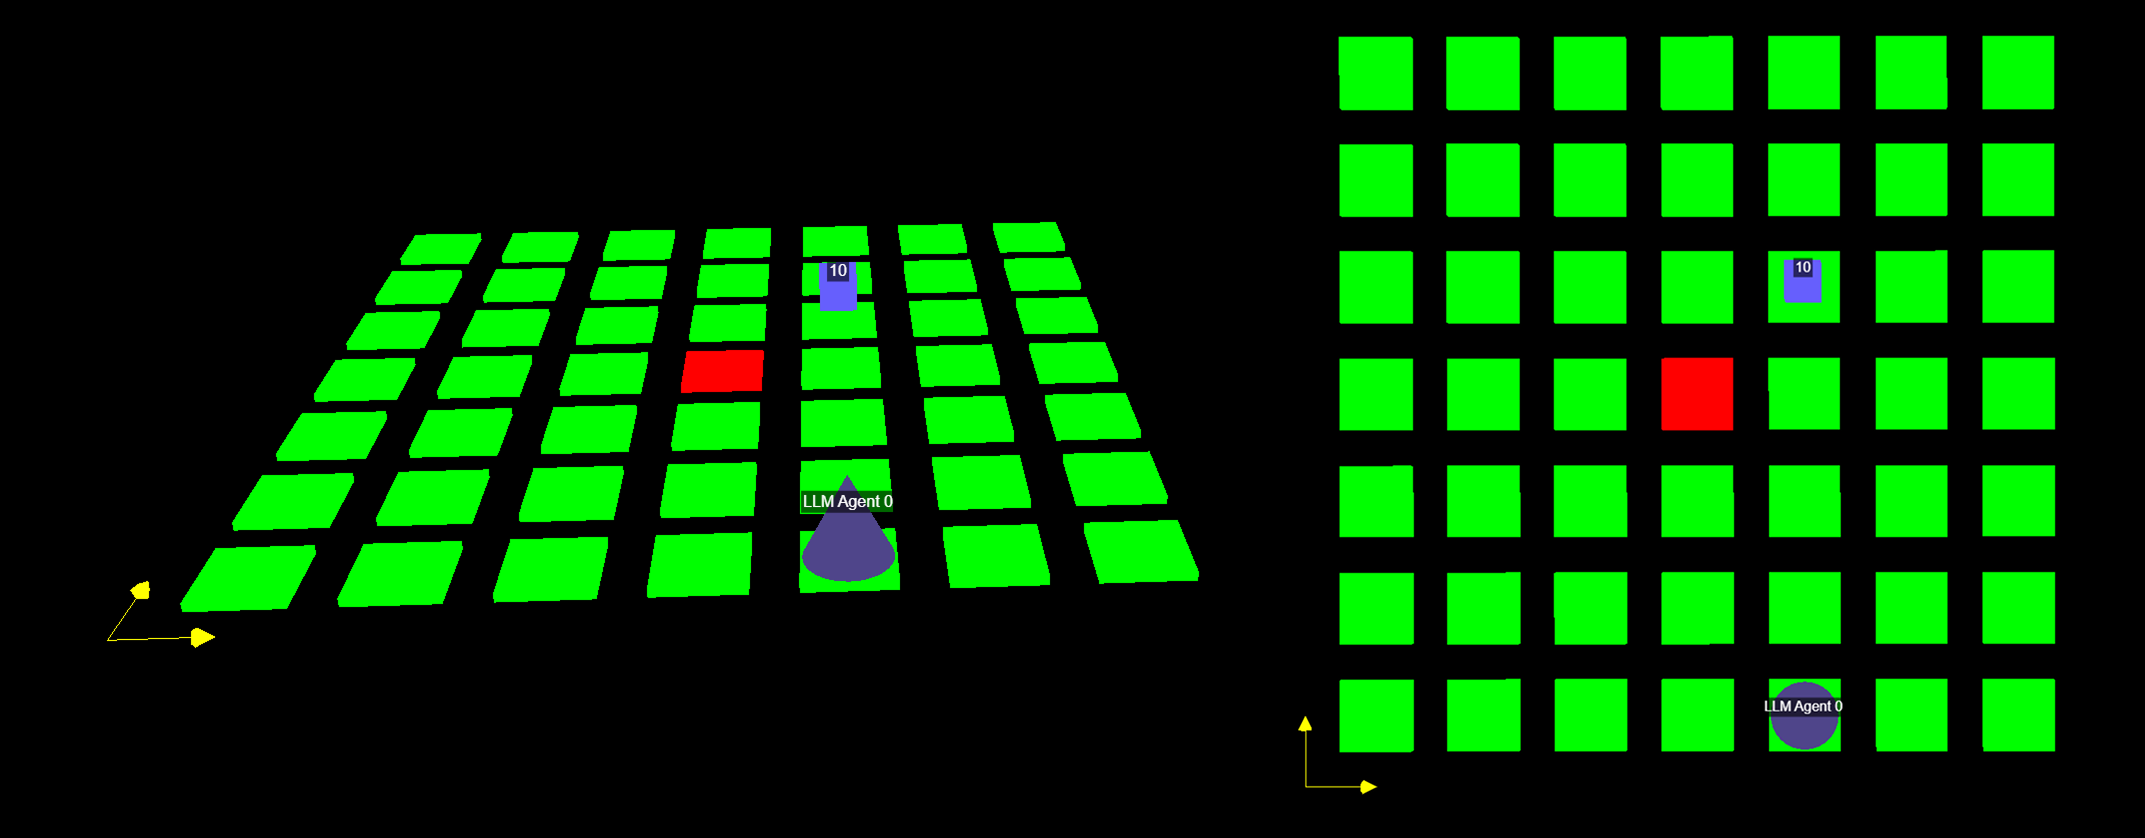
\includegraphics[width=0.90\textwidth]{
    images/experiment_setting/deliveroo_js.png
  }
  \caption{Two views of the same 7x7 Map in Deliveroo.js with a single central
  delivery zone.}
  \label{fig:deliveroo_js}
\end{figure}

The game can be played even by humans, by interacting in the browser; technically
speaking, it is a web-based platform consisting of three main components
connected to each other via sockets (implemented with Socket.io\footnote{\url{https://socket.io/}}):
\begin{itemize}
  \item \textbf{Game server}: it contains the entire logic of the game and it includes
    the implementation of client connection handler, parcel spawning, current environment
    status and so on;

  \item \textbf{Agent client}: it is the custom component that we developed to interact
    with the game server. It is a JavaScript file that connects to the server, manages
    all the logic of the agent (in our case, the LLM agent) and sends the
    actions to the server;

  \item \textbf{3D web app}: it is the visual representation of the game. It is
    a web page that connects to the server and receives the status of the game
    to render it in a 3D environment. It is not necessary for the agent to work,
    but it is useful to understand what is happening in the game.
\end{itemize}

As we can see from the Figure \ref{fig:deliveroo_js}, the game is a grid of
$N \times M$ tiles where the agent can move. Right now, the $(0, 0)$ cell is in
the bottom left corner. The map is defined in a JS file (example in Listing
\ref{lst:deliveroo_map_config}) where the number inside a cell represent the type
of the cell.

% \begin{lstlisting}[language=Python, caption={Example of a configuration for a 7x7 map with a single central delivery zone}, label={lst:deliveroo_map_config}]
\vspace{10mm}
\begin{codewindow}
  [JavaScript Code] \lstset{style=jsstyle, language=JavaScript, caption={Example of a 7x7 map with a single central delivery zone},
  label={lst:deliveroo_map_config}} \begin{lstlisting}
// 7x7 goal center deliver
module.exports = [
  [1, 1, 1, 1, 1, 1, 1],
  [1, 1, 1, 1, 1, 1, 1],
  [1, 1, 1, 1, 1, 1, 1],
  [1, 1, 1, 2, 1, 1, 1],
  [1, 1, 1, 1, 1, 1, 1],
  [1, 1, 1, 1, 1, 1, 1],
  [1, 1, 1, 1, 1, 1, 1],
];
\end{lstlisting}
\end{codewindow}
\vspace{10mm}

There are three possible types of cells:
\begin{itemize}
  \item \textcolor{primary}{\textbf{green}} (\texttt{1}): the agent can move on
    it. They can contain multiple parcels but only one agent at a time;

  \item \textcolor{red}{\textbf{red}} (\texttt{2}): the agent can move on it and
    deliver any number of parcel it has;

  \item \textcolor{black}{\textbf{black}} (\texttt{0}): the agent can't move on
    it and they can't contain any parcel (we will not use them in our tests).
\end{itemize}

The functioning is very straight forward:

\begin{itemize}
  \item \textbf{Agents}: there can be any number of agents that can cooperate or
    compete. Each agent has a score that is increased by delivering parcels. They
    are represented as cones with their name on it on the map (`LLM Agent' in
    Figure \ref{fig:deliveroo_js} is ours).

  \item \textbf{Parcels}: they are represented as small cubes with a number on it.
    The number is the reward the agent will get by delivering it. They spawn in random
    cells and they can be picked up by the agent. If they are not delivered in a
    certain amount of time, they may disappear.
\end{itemize}

% \begin{lstlisting} [language=Python, caption={Example of a configuration for the server}, label={lst:deliveroo_server_config}]

\subsection{Server Configuration and Event Handling}
\label{sub:server_configuration_event_handling}
\vspace{10mm}
\begin{codewindow}
  [JavaScript Code] \lstset{style=jsstyle, language=JavaScript, caption={Example of a configuration file for the server},
  label={lst:deliveroo_server_config}} \begin{lstlisting}
module.exports = {
  MAP_FILE: "map_file",

  PARCELS_GENERATION_INTERVAL: "5s",
  PARCELS_MAX: "1",

  MOVEMENT_STEPS: 1,
  MOVEMENT_DURATION: 50,
  AGENTS_OBSERVATION_DISTANCE: 100,
  PARCELS_OBSERVATION_DISTANCE: 100,
  AGENT_TIMEOUT: 100,

  PARCEL_REWARD_AVG: 10,
  PARCEL_REWARD_VARIANCE: "0",
  PARCEL_DECAYING_INTERVAL: "infinite",

  RANDOMLY_MOVING_AGENTS: 0,
  RANDOM_AGENT_SPEED: "2s",

  CLOCK: 50,
};
\end{lstlisting}
\end{codewindow}
\vspace{10mm}
The behavior of parcels in the system is defined through the server
configuration file. This file specifies key parameters that control parcel generation,
reward values, and decay over time. One such configuration is shown in the
example in Listing \ref{lst:deliveroo_server_config}.

Based on the server settings, a maximum number of parcels can be active simultaneously.
Each parcel is spawned at a fixed interval, with a random reward value determined
by a specified average and variance. Additionally, the configuration dictates whether
the reward remains constant or decreases over time.

In the example, parcels are generated every 5 seconds, but only one can exist at
a time. Each parcel starts with a reward value of exactly 10. Furthermore, since
\texttt{PARCEL\_DECADING\_INTERVAL} is set to \texttt{"infinite"}, the reward
does not decrease over time and the parcel will not disappear (until delivered).
This setup ensures a stable environment for testing the agent's performance.

The agent can interact with the environment using the following actions:
\begin{itemize}
  \item \textbf{up, down, left, right}: move in the specified direction, if the
    cell is empty and green or red;

  \item \textbf{pickup}: the agent can pickup a parcel in the cell it is in;

  \item \textbf{deliver}: the agent can drop a parcel in the cell it is in: if
    it is a delivery zone the parcel will disappear and the reward will be added
    to the player's score, otherwise it will just remain on the cell.
\end{itemize}

The server is responsible for transmitting events to the agent, ensuring that it
receives all relevant updates in real-time. Specifically, the following events
were utilized in our tests:

\begin{itemize}
  \item \texttt{onMap} (width, height, tiles): it sends the width and the height
    of the map, along with all the tiles in it. Tiles are currently sent as a dictionary
    \{\texttt{x: INT, y: INT, delivery: BOOL, spawner: BOOL}\} where \texttt{delivery}
    is true if the tile is a delivery zone and \texttt{spawner} is true if a
    parcel can spawn on it;

  \item \texttt{onYou} (id, name, x, y, score ): it sends the id, the name, the
    x and y coordinates and the score of the agent connected that the code is
    piloting;

  \item \texttt{onParcelsSensing} async (perceived\_parcels): it is an async function
    that sends the parcels that the agent can see at any time. The parcels are
    sent as a dictionary \{\texttt{x: INT, y: INT, reward: INT}\} where \texttt{x}
    and \texttt{y} are the coordinates of the parcel and \texttt{reward} is the
    reward the agent will get by delivering it.
\end{itemize}

\section{Large Language Models Selection}
\label{sec:llm_models}

As mentioned in Section \ref{sec:large_language_models_llms}, Large Language Models
are powerful tools that have revolutionized the field of natural language processing.
The way they generate text based on input prompts has opened up new
possibilities for research and applications in various domains.

One of the core aspects of LLMs is their autoregressive nature, meaning they generate
text one token at a time (given the current implementation, but alternative solution
are currently being studied, for example by Meta AI\footnote{\url{https://ai.meta.com/}}
in the paper `Better \& Faster Large Language Models via Multi-token Prediction'
by Gloeckle et al.\cite{gloeckle2024betterfasterlarge}), predicting the next most
likely token based on the context provided. This capability is what allows LLMs
to generate coherent and contextually relevant responses. The way these systems operate
can be broken down into a (simplified) step-by-step process:

\begin{itemize}
  \item The prompt (the request) is tokenized, which means it is divided into
    smaller units called tokens. These tokens are predefined character combinations
    that serve as the building blocks for processing text. An example of this
    tokenization process is illustrated in Figure \ref{fig:tokenization_example}.
    Once tokenized, the prompt is passed to the model for processing;

  \item The model then generates the ``next token" based on a probability
    distribution computed using attention mechanisms, to determine the most contextually
    appropriate next token;

  \item The newly generated token is appended to the existing sequence, and the
    process is repeated iteratively. This continues until a predefined stopping criterion
    is met, either reaching a maximum token limit or encountering a special
    termination token.
\end{itemize}

\begin{figure}[h!]
  \centering
  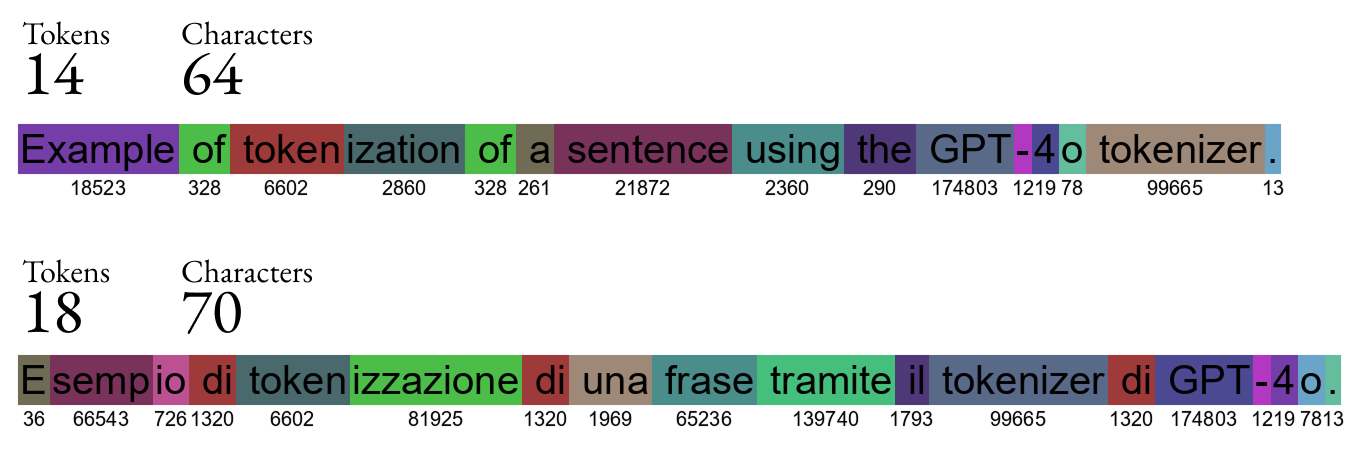
\includegraphics[width=0.88\textwidth]{
    images/experiment_setting/tokenization_example.png
  }
  \caption{Example of tokenization of a sentence using the GPT-4o tokenizer.}
  {\emph{Source: Data from OpenAI Platform}\footnotemark} \label{fig:tokenization_example}
\end{figure}
\footnotetext{{\url{https://platform.openai.com/tokenizer}}}

One key element of this process is how the next token is selected. The winning
token is picked from a probability distribution obtained through the softmax
function. However, if selection were purely deterministic, the model would always
generate the same output given the same prompt, making it rigid and predictable.
To introduce variability and prevent repetitive patterns, a controlled amount of
randomness is introduced using the \texttt{temperature} parameter.

The temperature parameter plays a crucial role in regulating randomness in text generation:
this mechanism explains why the same prompt can yield different outputs when
used multiple times: because the token selection is influenced by this controlled
randomness.

Beyond temperature, another factor that influences token selection is the logit
bias\footnote{\url{https://www.vellum.ai/llm-parameters/logit-bias}}. Logit bias
allows direct intervention in the probability of specific tokens being chosen
during text generation. Instead of relying solely on the model's learned probabilities,
users can manually adjust the likelihood of certain tokens appearing by
modifying the logits (the unnormalized probabilities) before applying the
softmax function.

The logit bias mechanism operates as follows:

\begin{itemize}
  \item Positive bias values increase the probability of a specific token being selected,
    making it more likely to appear in the generated text.

  \item Negative bias values decrease the probability of a token, potentially
    eliminating it from consideration altogether.
\end{itemize}

This approach gives users more control over text generation, allowing them to
guide the model toward preferred outputs while avoiding undesired words or
phrases. A simplified implementation of how logit bias works can be seen in the Python
code snippet in Listing \ref{lst:logit_bias}, where we want to increase the
likelihood of the word ``fox'' and decrease the likelihood of the word ``quick''.

\vspace{10mm}
\begin{codewindow}
  [Python Code] \lstset{style=pythonstyle, language=Python, caption={Example of what a basic implementation of logit bias could look like},
  label={lst:logit_bias}} \begin{lstlisting}
[...]

# Get the logits (raw predictions)
outputs = model(**inputs)
logits = outputs.logits

logit_bias = {
  # Decrease likelihood for the word "quick"
  tokenizer.encode("quick")[0]: -2.0,
  # Increase likelihood for the word "fox"
  tokenizer.encode("fox")[0]: 2.0,
  # Almost never generate the word "slow"
  tokenizer.encode("slow")[0]: -100.0,
  # Almost always generate the word "brown"
  tokenizer.encode("brown")[0]: 100.0,
}

# Apply logit bias: modify logits of specific tokens
for token_id, bias in logit_bias.items():
  logits[token_id] += bias

# Convert logits by applying softmax
probs = torch.nn.functional.softmax(logits, dim=-1)

[...]
\end{lstlisting}
\end{codewindow}
\vspace{10mm}

This technique is particularly useful in scenarios where the generated text must
adhere to specific constraints. For example, logit bias can be used for content moderation,
ensuring that the model avoids generating harmful, offensive, or inappropriate
content. By assigning a strong negative bias to certain tokens used to build specific
words or sentences, users can effectively steer the model away from producing
undesirable responses.

Not only, there are some cases where an LLM has been expanded with custom and private
information, via fine-tuning or Retrieval Augmented Generation (as we cited in Section
\ref{sub:llms_uncertainty}). In this context, we may want to force the model to
not generate some specific content that may be useful for the overall response
but should not be shared.

On the other hand, logit bias can be leveraged to override built-in model safeguards.
In some cases, AI models have safety mechanisms that prevent them from answering
certain types of questions, responding with phrases like ``I'm sorry, but I can't
provide that information." By applying a negative logit bias to the tokens that generate
the words that build this response, users can force the model to produce an
alternative reply, whether it be a reworded refusal or even an answer to the original
question.

Overall, logit bias is a powerful tool for modelling model behavior, allowing developers
to enforce preferred linguistic patterns, avoid specific terminology, and customize
AI responses according to their needs. When combined with temperature
adjustments and other generation techniques, it provides a robust framework for controlling
LLM output and ensuring its alignment with desired objectives.

\subsection{Open Source Models}

The term ``Large" in Large Language Models (LLMs) refers to their extensive number
of parameters and the vast datasets used during training. Training these models
is a resource-intensive process, both in terms of computational power and time.
However, some organizations choose to release their models as open source,
allowing the community to access and utilize them freely. This approach is also beneficial
the broader AI community, as it fosters innovation: if a new open source model is
released and it's ``the most powerful", it sets a new baseline for companies.
This compels them to find further innovations, either by reducing costs or developing
even more powerful models with new features.

In the context of LLMs, the term ``open source" differs from its traditional usage
in software development\footnote{\url{https://promptengineering.org/llm-open-source-vs-open-weights-vs-restricted-weights/}}.
Specifically, there is a nuanced distinction that categorizes publicly available
models into two primary types:

\begin{itemize}
  \item \textbf{Open Source}: The creators provide full access to the model's source
    code, architecture, training data, and pre-trained weights. This level of transparency
    allows users to understand, modify, and enhance the model comprehensively.

  \item \textbf{Open Weights}: The creators make the model's pre-trained weights
    publicly available but may withhold other critical components, such as the
    training data or detailed methodologies used during training. This approach enables
    users to employ the model for specific tasks but limits their ability to fully
    comprehend or modify its underlying structure.
\end{itemize}

In the following subsections, we will present some open models we tested in the
early stages of our research. The results analyzed in Chapter \ref{cha:results_discussion}
do not consider these models due to certain limitations, which we will discuss
shortly. Nonetheless, they are worth mentioning as they provided a valuable
starting point during the initial phases of our project.

\subsubsection{Challenges with Open Source Models}

One significant challenge we encountered with open source models was the implementation
of the logit bias mechanism. While the example in Listing \ref{lst:logit_bias}
may suggest simplicity, the reality is more complex. Implementing this mechanism
requires:

\begin{itemize}
  \item Reconstructing the model's architecture accurately.

  \item Loading the pre-trained weights appropriately.

  \item Modifying the model's intricate structure to extract the raw values and change
    them to incorporate the logit bias.
\end{itemize}

These steps demand substantial time, and in addition, running those models locally
requires large computational resources; all of this for something not essential
to the core objectives of our project (since closed models provide this feature out
of the box).

Moreover, during initial tests, we observed difficulties in constraining the
Open Source models to produce specific tokens from a list without altering the
logit bias. For instance, when prompted to ``Answer with just a single letter
between U, D, L, R." (the explanation for this prompt will be given in Section
\ref{sec:prompt_creation_choices}) the model often responded with full sentences
like "Sure, the answer is U!". Truncating such responses to a single token would
result in outputs like ``Sure" which is not the desired outcome. This is a
problem that we didn't have with the closed source models, that we will discuss in
the next sub-section \ref{sub:closed_source_models_openai}.

So, open source models have been tested only in the first instance of the
project, to test the logic of the agent without wasting credit with OpenAI API.

They have been run through Ollama\footnote{\url{https://ollama.com/}}, a tool for
running and managing large language models locally. It simplifies downloading, running,
and interacting with models without relying on cloud services.

\subsubsection{LLaMa 3.2}

\begin{wrapfigure}
  [10]{l}{.22\textwidth}
  \centering
  \def\stackalignment{l}\stackunder{ 
\includegraphics[width=\linewidth]{images/experiment_setting/meta.png} }
  {\scriptsize \parbox[t]{\linewidth}{Source: \href{https://www.flaticon.com/free-icon/meta_6033716}{Meta icons created by Freepik - Flaticon}}}
\end{wrapfigure}

LLaMa 3.2, developed by Meta AI\footnote{\url{https://ai.meta.com/blog/llama-3-2-connect-2024-vision-edge-mobile-devices/}},
is a multimodal large language model designed to process both textual and visual
data, marking Meta's first open-source AI model with such capabilities. The model
is available in two configurations: an 11-billion-parameter version and a more
robust 90-billion-parameter variant. There are also a 1-billion-parameter and 3-billion-parameter
text-only versions of the models. These models are optimized for deployment on
mobile (yet powerful) hardware platforms.

The model tested in our experiments was the \emph{text-only 3-billion-parameter}
version.
\vspace{8mm}
\subsubsection{Gemma 2}
\begin{wrapfigure}
  [8]{l}{.22\textwidth}
  \centering
  \def\stackalignment{l}\stackunder{ 
\includegraphics[width=\linewidth]{images/experiment_setting/gemma.png} }
  {\scriptsize \parbox[t]{\linewidth}{Source: \href{https://logowik.com/google-gemma-ai-logo-vector-71178.html}{logowik}}}
\end{wrapfigure}
Gemma 2, introduced by Google\footnote{\url{https://developers.googleblog.com/en/gemma-explained-new-in-gemma-2/}},
is an open suite of language models available in parameter sizes of 2 billion, 9
billion, and 27 billion. The 27-billion-parameter model has demonstrated
exceptional performance, surpassing larger models in real-world conversational benchmarks.
This suite is built upon the same research and technology that underpins Google's
Gemini models, emphasizing both performance and accessibility.

The model tested in our experiments was the \emph{9-billion-parameter} version.

\vspace{1mm}
\subsubsection{DeepSeek-V3}
\begin{wrapfigure}
  [9]{l}{.22\textwidth}
  \centering
  \def\stackalignment{l}\stackunder{ 
\includegraphics[width=\linewidth]{images/experiment_setting/ds.png} }
  {\scriptsize \parbox[t]{\linewidth}{Source: \href{https://github.com/deepseek-ai}{DeepSeek GitHub}}}
\end{wrapfigure}
DeepSeek-V3, developed by DeepSeek \footnote{\url{https://github.com/deepseek-ai/DeepSeek-V3}},
is a Mixture-of-Experts (MoE) language model comprising a total of 671 billion
parameters, with 37 billion activated per token during inference. It employs
Multi-head Latent Attention (MLA) and the DeepSeekMoE architecture to achieve
efficient inference and cost-effective training. The model was pre-trained on 14.8
trillion diverse and high-quality tokens, followed by supervised fine-tuning and
reinforcement learning stages to fully harness its capabilities. Despite its extensive
scale, DeepSeek-V3's training process is notably efficient and it has
demonstrated remarkable stability throughout training. Comprehensive evaluations
reveal that DeepSeek-V3 outperforms other open-source models and achieves performance
comparable to leading closed-source models.

Unfortunately, we didn't get to test it because it released after the end of the
project, but it is worth mentioning for future research thanks to its impressive
performance.

\subsection{Closed Source Models - OpenAI}
\label{sub:closed_source_models_openai}

Before delving into the specifics of this section, we want to emphasize that OpenAI
is not the only company offering closed-source AI models. Several other
providers exist, such as Anthropic\footnote{\url{https://www.anthropic.com/}}, which
develops the Claude family of models, but also DeepSeek\footnote{\url{https://api-docs.deepseek.com/}},
that developed the open source DeepSeek-V3 provides API access to its models as
well.

While OpenAI remains the most widely recognized and utilized provider, particularly
in research and industry applications, it is important to acknowledge that many
of the benefits and drawbacks of closed-source models apply broadly across all
such services. Nevertheless, since our work specifically relies on OpenAI's
models, our discussion will primarily focus on them while keeping in mind that similar
considerations extend to other closed-source alternatives.

\vspace{1mm}

A key distinction between open-source and closed-source models is the
transparency regarding their architecture. In many closed-source models, details
such as the exact number of parameters are not publicly disclosed. For instance,
while OpenAI's GPT-3\cite{brown2020languagemodelsfewshotlearners} is known to have
a maximum of 175 billion parameters\footnote{\url{https://en.wikipedia.org/wiki/GPT-3}},
the parameter counts for subsequent models like GPT-4\cite{openai2024gpt4technicalreport}
have not been officially confirmed. Estimates suggest that GPT-4 may have around
1.76 trillion parameters, but this remains speculative\footnote{\url{https://en.wikipedia.org/wiki/GPT-4}}.

\begin{wrapfigure}
  [11]{r}{.22\textwidth}
  \centering
  \def\stackalignment{r}\stackunder{ 
\includegraphics[width=\linewidth]{images/experiment_setting/openai.png} }
  {\scriptsize \parbox[t]{\linewidth}{Source: \href{https://www.vecteezy.com/png/22227364-openai-chatgpt-logo-icon}{Vecteezy}}}
\end{wrapfigure}

OpenAI was established as a research organization dedicated to advancing
artificial intelligence. They initially released models such as GPT-2\cite{Radford2019LanguageMA}
and Whisper\cite{radford2022robustspeechrecognitionlargescale} (a speech
recognition model) to the public at no cost. GPT-2, for example, was made
available with various model sizes, the largest containing 1.5 billion parameters\footnote{\url{https://en.wikipedia.org/wiki/GPT-2}}.

Subsequently, OpenAI developed GPT-3 and DALL·E\cite{ramesh2021zeroshottexttoimagegeneration},
introducing them through a commercial platform and API services. The landscape
of AI applications shifted significantly with the release of ChatGPT, a conversational
AI model that garnered widespread attention for its advanced language understanding
and generation capabilities.

OpenAI offers access to their models via subscription plans and a pay-as-you-go API,
with pricing varying based on the specific model utilized. The API provides granular
control over model behavior through parameters such as \texttt{logit\_bias}, that,
as the name suggests, allows users to adjust the likelihood of specific tokens appearing
in the generated output by assigning bias values ranging from -100 to 100.

However, a limitation of closed-source models is the lack of transparency
regarding updates or changes. Users may be unaware of modifications that could affect
model behavior. For instance, there have been instances where the behavior of the
logit\_bias parameter changed without prior (or ``at run-time") notice. We have identified
three primary behaviors that the logit\_bias parameter can have depending on the
version of the API, which appears to be independent from any update of the
models themselves:
\begin{enumerate}
  \item \textbf{No change}: The API does not apply the logit\_bias at all,
    resulting in outputs identical to those generated without using the
    parameter;

  \item \textbf{Exclusive}: The logit\_bias is applied strictly. Setting a token's
    bias to 100 forces the model to produce that token; if multiple tokens are set
    to 100, the model will choose among them. Conversely, setting a token's bias
    to -100 prevents that token from appearing in the output;

  \item \textbf{Soft}: The logit\_bias is applied moderately. Assigning a token
    a bias of 100 significantly increases its likelihood of being produced, but other
    tokens may still be selected. Similarly, setting a token's bias to -100
    greatly decreases its likelihood, but it may still appear.
\end{enumerate}

Our tests were conducted during a period when the API exhibited the third
behavior (Soft). However, due to frequent API updates, we cannot guarantee the reproducibility
of these results. To more mitigate variability, we set the temperature parameter
to zero during our tests, aiming for deterministic outputs. To limit the impact of
unwanted tokens appearing in the output or vice versa, we decided to ignore any
token that was not in the list of expected tokens and we assigned to the missing
tokens the 20th log-probability minus the 19th one.

Another crucial feature offered by OpenAI is the \texttt{logprobs} parameter.
When specified, this parameter returns the log probabilities of the top tokens that
the model may generate as the ``next token".

This information is essential for computing the uncertainty of the model's
predictions, as detailed in Section \ref{ssub:tokens_log_probability}. It's
important to note that also the behavior of the \texttt{logprobs} parameter can change
over time. For instance, when the paper `Robots That Ask For Help: Uncertainty Alignment
for Large Language Model Planners' was released, the \texttt{logprobs} parameter
returned a maximum of 5 tokens. Since then, this limit has been increased to a
maximum of 20 tokens. In the future, it may be adjusted again, so it's important
to keep this in mind when working with the API.

Pricing per 1 million tokens for all the OpenAI models used can be seen in Table
\ref{tab:pricing}; the functioning of caching is explained in Section
\ref{sec:prompt_creation_choices}.

\vspace{3mm}
\begin{table}[h]
  \centering
  \renewcommand{\arraystretch}{1.5}
  \setlength{\tabcolsep}{8pt}
  \begin{tabular}{ c c c c }
    \textbf{Model} & \textbf{Input} & \textbf{Cached Input} & \textbf{Output} \\
    \hline
    gpt-4o-mini    & \$0.15         & \$0.075               & \$0.60          \\
    gpt-4o         & \$2.50         & \$1.25                & \$10.00         \\
    gpt-3.5-turbo  & \$0.50         & /                     & \$1.50          \\
  \end{tabular}
  \caption{Pricing Table per 1Mil tokens for the tested models.}
  {\emph{Source: OpenAI \footnotemark}} \label{tab:pricing}
\end{table}
\footnotetext{\url{https://platform.openai.com/pricing}}
\vspace{3mm}

\subsubsection{GPT-4o-mini}
GPT-4o-mini, developed by OpenAI\footnote{\url{https://openai.com/research/gpt-4o}},
is a lightweight variant of the GPT-4o architecture, optimized for efficiency while
maintaining strong performance across a range of tasks. It is designed to
deliver fast inference and lower computational costs, making it suitable for deployment
in real-time applications and on-device AI systems. While OpenAI has not
publicly disclosed the parameter count, it is positioned as a more efficient alternative
to larger models in the GPT-4 family.

The main model used for the tests in our experiments was indeed GPT-4o-mini,
selected for its balance of performance and pricing.

\subsubsection{GPT-4o}
GPT-4o is OpenAI's flagship multimodal model, capable of processing and generating
text, images, and audio in real time. It represents a significant leap in
efficiency and latency, outperforming previous iterations such as GPT-4-turbo while
operating at a lower computational cost. Unlike its predecessors, GPT-4o is natively
trained across multiple modalities rather than combining separate models for different
inputs. Though OpenAI has not released detailed architectural specifications, benchmark
results indicate substantial improvements in reasoning, multilingual proficiency,
and response speed.

It has been used less than GPT-4o-mini because of the higher cost and the fact that,
since from the first tests, the results were almost identical to the mini version.

\paragraph{AzureAPI}
\label{par:azureapi} GPT-4o was accessed via the Azure OpenAI API, provided by the
University of Trento, offering a secure and private interface for interacting
with the model. To facilitate communication between the agent's JavaScript code and
the API, a lightweight Python server was developed. The server's code is available
on GitHub\footnote{\url{https://github.com/davidemodolo/master_thesis_project/blob/main/azureAPI/server.py}}.

\subsubsection{GPT-3.5-turbo}
GPT-3.5-turbo is a high-performance variant of OpenAI's GPT-3.5 model. It provides
strong general-purpose capabilities while being more accessible for applications
requiring large-scale deployment. Though it does not match GPT-4-level reasoning
abilities, it remains competitive in many NLP benchmarks and is widely used for production
AI services.

Unfortunately, this model has been the weakest in our tests; we will discuss this
in depth in the Section \ref{sec:models_comparison}.